%\begin{landscape}% Landscape page



\section{ Comparação entre as modelagens}

\subsection{Comparação atendimento de requisição}
\begin{figure}[!h]
\caption{Gerencia de requisição - AS-IS}
\centering % para centralizarmos a figura
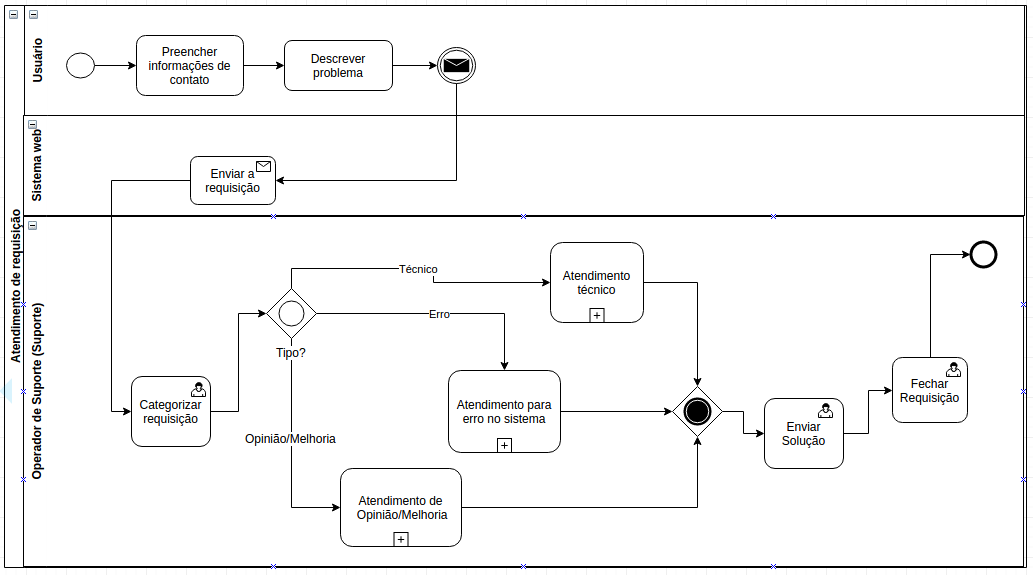
\includegraphics[width=15cm,height=6cm]{as-is/01_atendimento_de_requisicao.png}
\label{figura:atendimento_requisicao_as_is}
\end{figure}


\begin{figure}[!h]
\caption{Gerencia de requisição- TO-BE}
\centering % para centralizarmos a figura
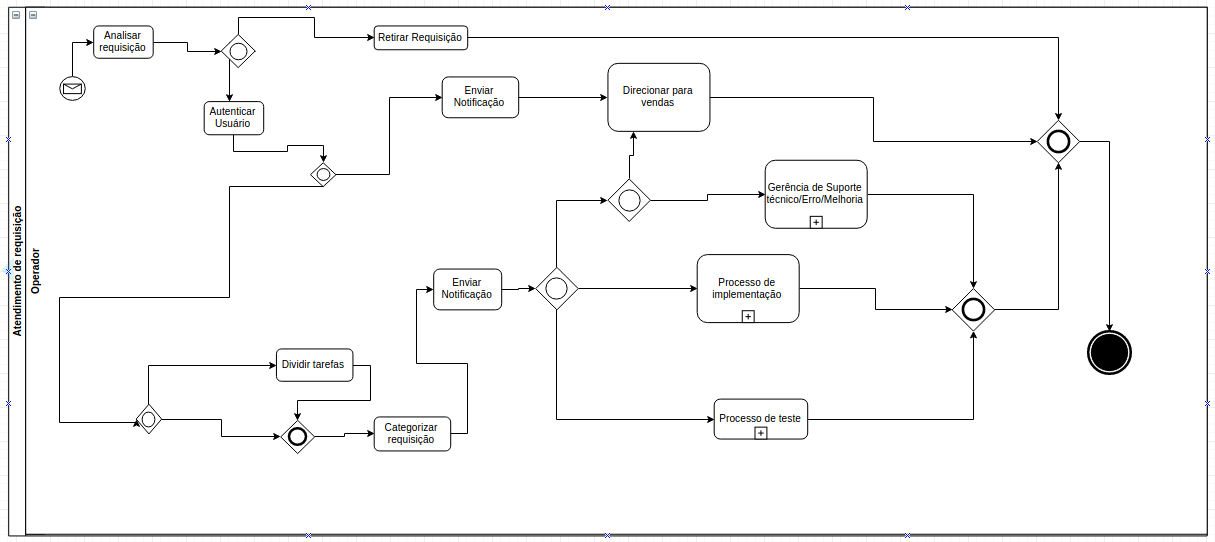
\includegraphics[width=16cm,height=7cm]{to_be/01_atendimento_de_requisicao.png}
\label{figura:atendimento_requisicao_to_be}
\end{figure}

\clearpage

\subsection{Comparação atendimento técnico}

\begin{figure}[!h]
\caption{Atendimento técnico - AS-IS}
\centering % para centralizarmos a figura
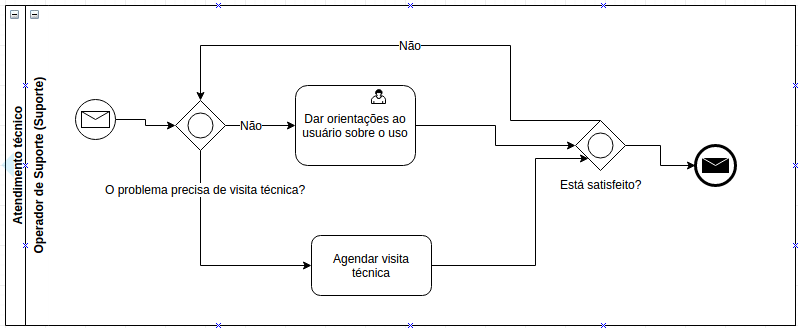
\includegraphics[width=15cm]{as-is/02_atendimento_tecnico.png}
\label{figura:suporte_tecnico_as_is}
\end{figure}

\begin{figure}[!h]
\caption{Atendimento técnico - TO-BE}
\centering % para centralizarmos a figura
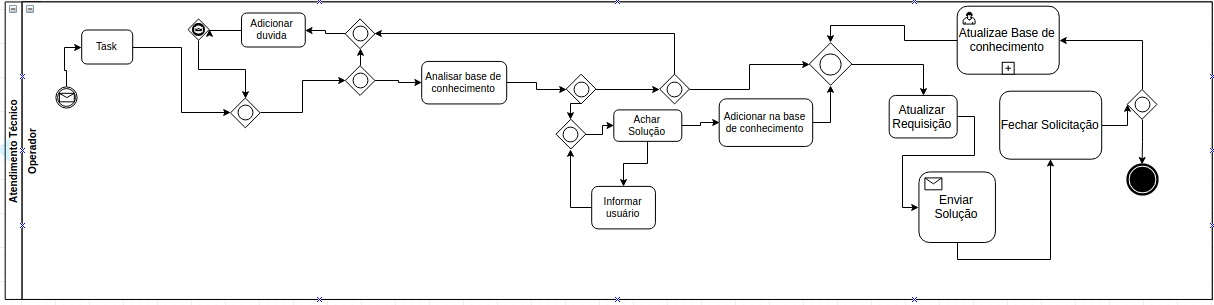
\includegraphics[width=16cm,height=7cm]{to_be/02_atendimento_tecnico.png}
\label{figura:suporte_tecnico_to_be}
\end{figure}

\clearpage
\subsection{Comparação atendimento para erro no sistema}

\begin{figure}[!h]
\caption{Atendimento para erro no sistema - AS-IS}
\centering % para centralizarmos a figura
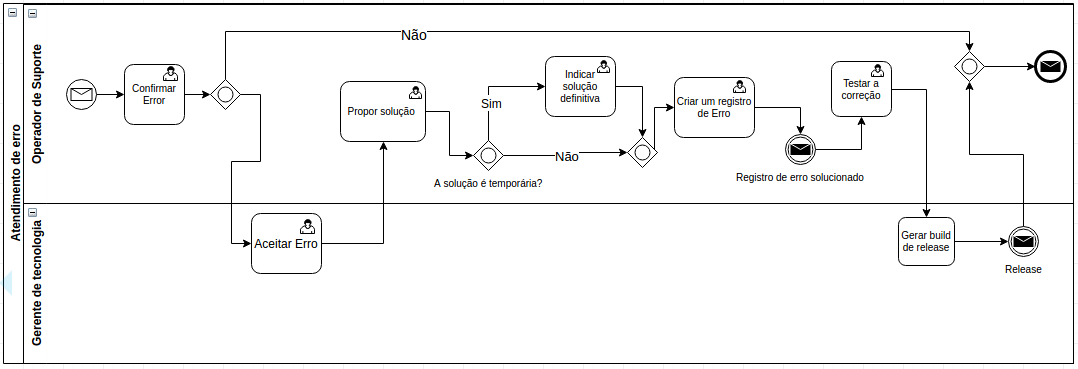
\includegraphics[width=16cm, height=7cm]{as-is/03_atendimento_de_erro.png}
\label{figura:atendimento_de_erro_as_is}
\end{figure}


\begin{figure}[!h]
\caption{Atendimento para erro no sistema - TO-BE}
\centering % para centralizarmos a figura
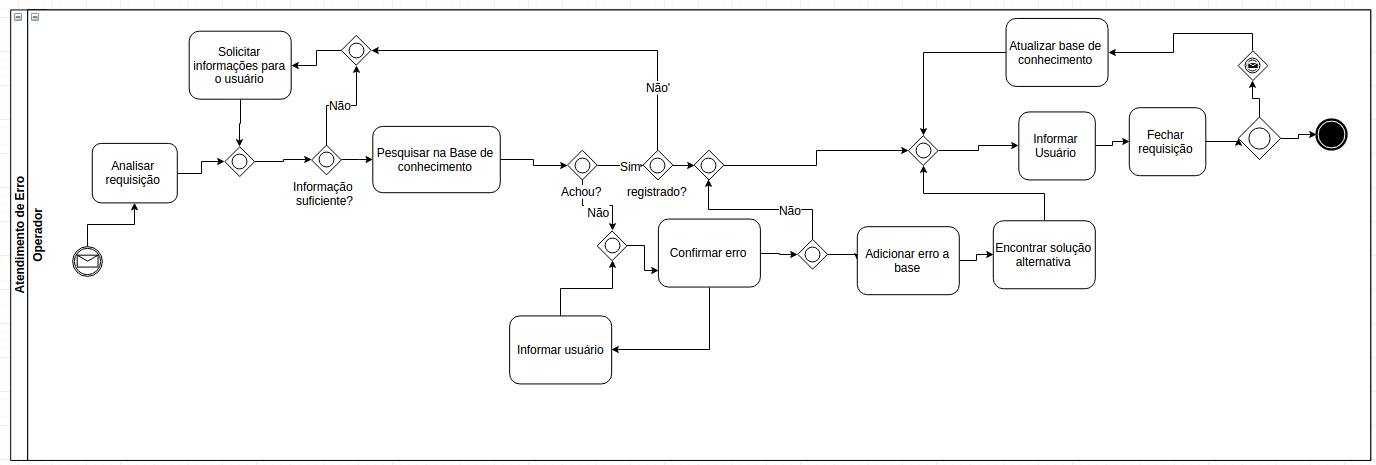
\includegraphics[width=16cm,height=7cm]{to_be/03_atendimento_de_erro.png}
\label{figura:atendimento_de_erro_to_be}
\end{figure}

\clearpage% Flush page


\subsection{Comparação Atendimento de Opinião/Melhoria}

\begin{figure}[!h]
\caption{Atendimento de Opinião/Melhoria - AS-IS}
\centering % para centralizarmos a figura
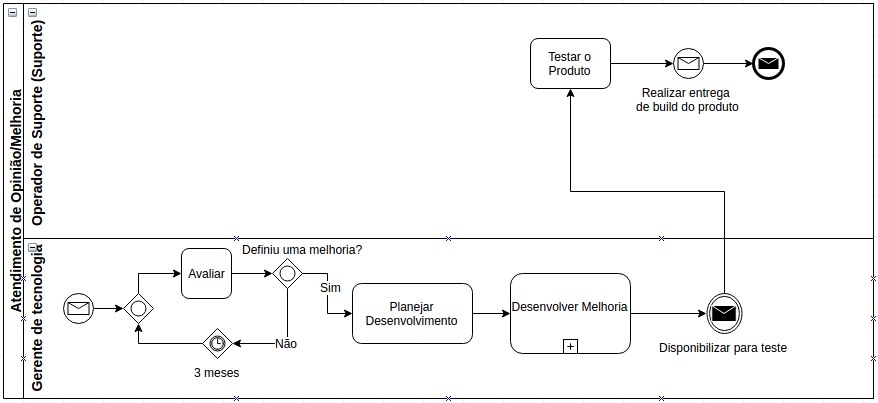
\includegraphics[width=15cm,height=7cm]{as-is/04_atendimento_de_melhoria.png}
\label{figura:atendimento_de_melhoria_as_is}
\end{figure}

\begin{figure}[!h]
\caption{Atendimento para erro no sistema -  TO-BE}
\centering % para centralizarmos a figura
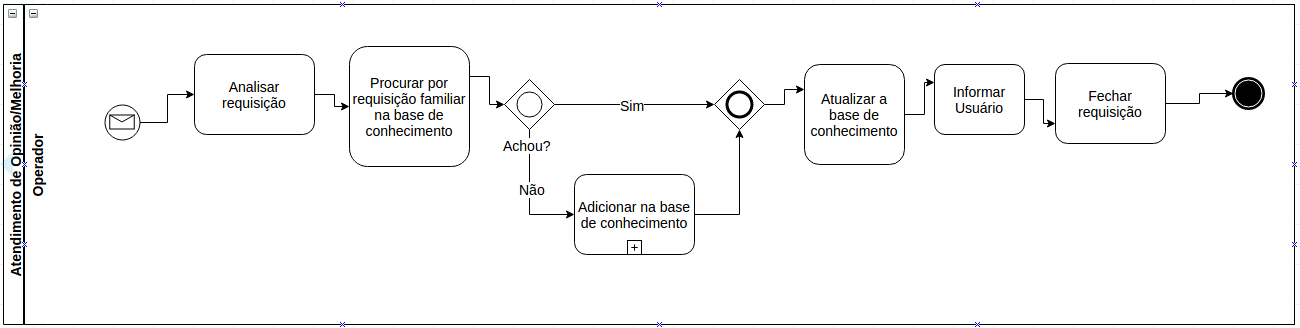
\includegraphics[width=15cm,height=7cm]{to_be/04_atendimento_de_melhoria.png}
\label{figura:atendimento_de_erro_to_be}
\end{figure}
